\documentclass{beamer}
\usetheme{metropolis}
\usepackage{graphicx}
\usepackage{subfig}
\usepackage{tcolorbox}
\title{Algebra-Based Physics: Electricity, Magnetism, and Modern Physics (PHYS135B): Unit 2}
\author{Jordan Hanson}
\institute{Whittier College Department of Physics and Astronomy}

\begin{document}
\maketitle

\section{Summary}

\begin{frame}{Unit 2 Summary}
\textbf{Reading: Chapters 21.1 - 21.4, 21.6}
\begin{enumerate}
\item Resistors in series and parallel
\item Electromotive force (EMF) and terminal voltage
\item Kirchhoff's rules
\item Voltmeters and ammeters
\item RC circuits
\end{enumerate}
\end{frame}

\section{Resistors in Series and Parallel}

\begin{frame}{Resistors in Series and Parallel, EMF}
\textbf{\alert{Series and parallel}} resistances change how current and power flow in a circuit.
\begin{figure}
\centering
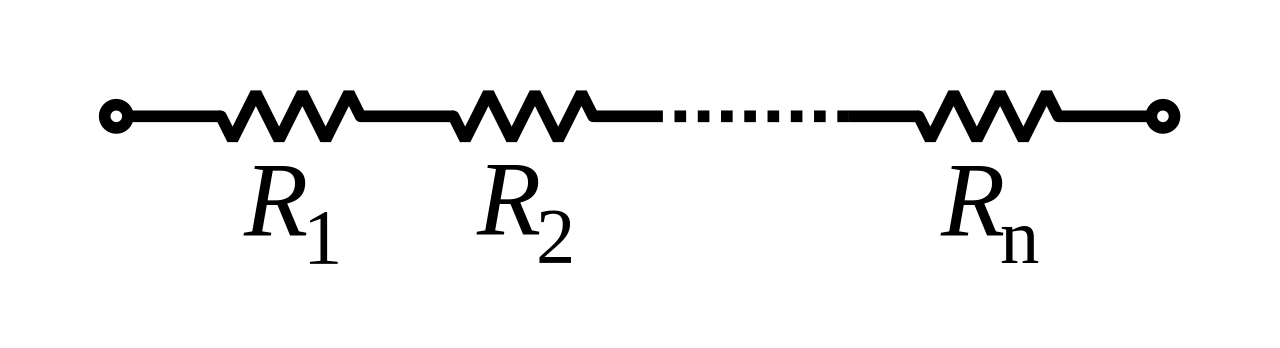
\includegraphics[width=0.5\textwidth]{figures/series_resist.png}
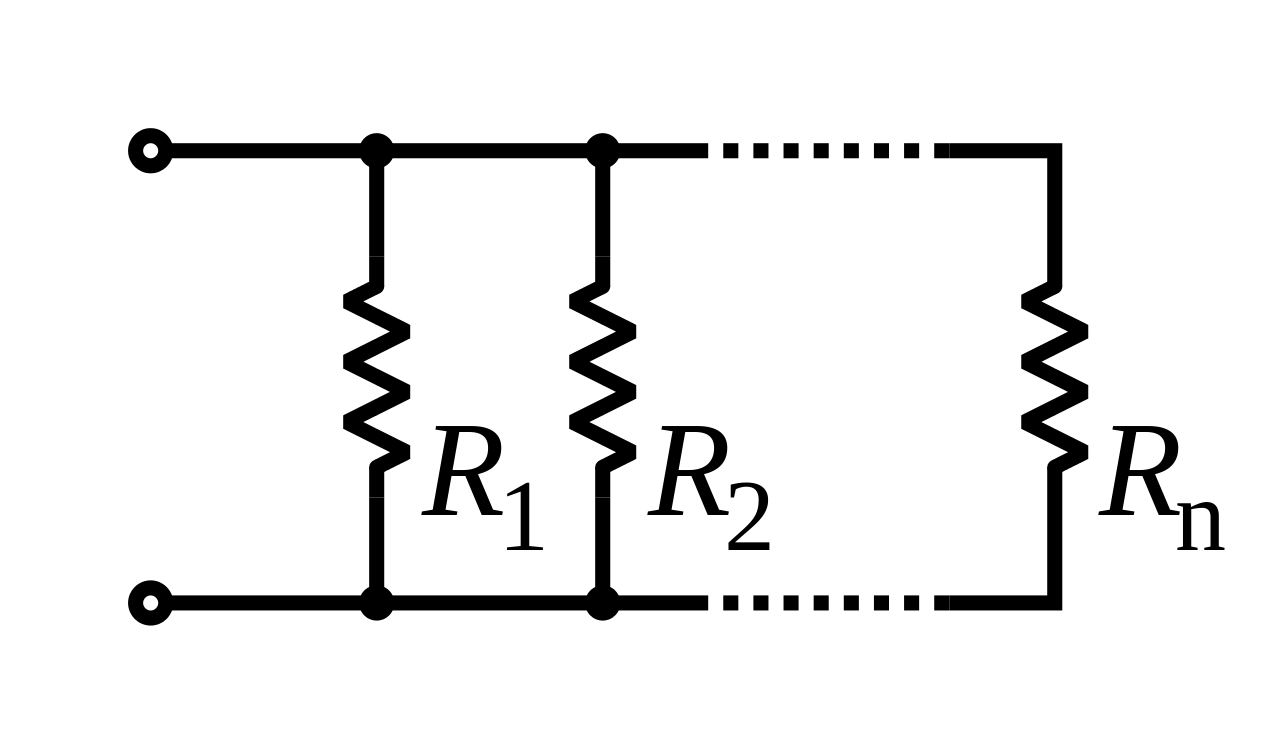
\includegraphics[width=0.4\textwidth]{figures/parallel_resist.png}
\caption{\label{fig:series_and_parallel} (Left) Resistors in series. (Right) Resistors in parallel.}
\end{figure}
\end{frame}

\begin{frame}{Resistors in Series and Parallel}
\footnotesize
\textbf{\alert{Series}} resistances:
\begin{itemize}
\item Share one current
\item Represent different voltage changes
\end{itemize}
\begin{figure}
\centering
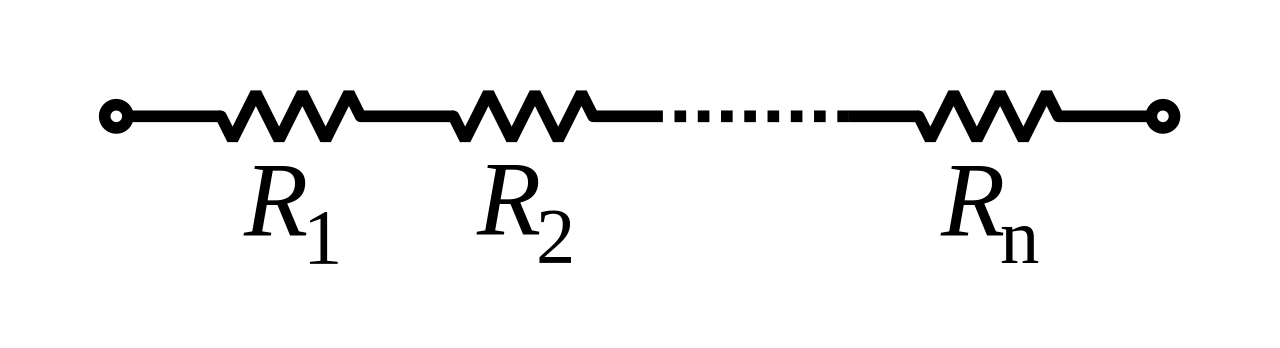
\includegraphics[width=0.5\textwidth]{figures/series_resist.png}
\caption{\label{fig:series} Resistors in series.}
\end{figure}
\begin{align}
q\Delta V_{\rm tot} &= q\Delta V_{\rm 1} + q\Delta V_{\rm 2} + ... + q\Delta V_{\rm n} \\
\Delta V_{\rm tot} &= \Delta V_{\rm 1} + \Delta V_{\rm 2} + ... + \Delta V_{\rm n} \\
I R_{\rm tot} &= I R_{\rm 1} + I R_{\rm 2} + ... + I R_{\rm n} \\
R_{\rm tot} &= R_{\rm 1} + R_{\rm 2} + ... + R_{\rm n}
\end{align}
\end{frame}

\begin{frame}{Resistors in Series and Parallel}
\footnotesize
\textbf{\alert{Parallel}} resistances:
\begin{itemize}
\item Share one voltage
\item Represent different currents
\end{itemize}
\begin{figure}
\centering
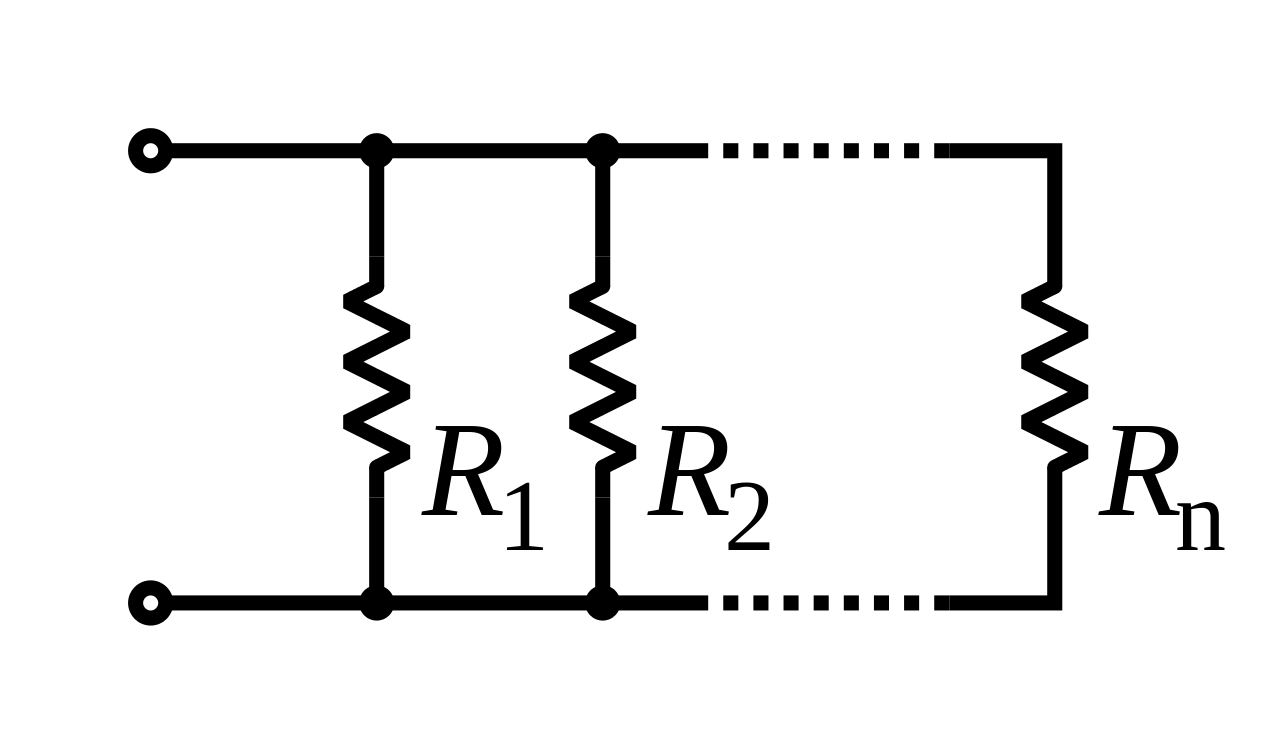
\includegraphics[width=0.3\textwidth]{figures/parallel_resist.png}
\caption{\label{fig:parallel} Resistors in parallel.}
\end{figure}
\begin{align}
I_{\rm tot} &= I_{\rm 1} + I_{\rm 2} + ... + I_{\rm n} \\
\frac{\Delta V}{R_{\rm tot}} &= \frac{\Delta V}{R_{\rm 1}} + \frac{\Delta V}{R_{\rm 2}} + ... + \frac{\Delta V}{R_{\rm n}} \\
\frac{1}{R_{\rm tot}} &= \frac{1}{R_{\rm 1}} + \frac{1}{R_{\rm 2}} + ... + \frac{1}{R_{\rm n}}
\end{align}
\end{frame}

\begin{frame}{Resistors in Series and Parallel}
\textbf{\alert{Series}} resistances:
\begin{equation}
\boxed{R_{\rm tot} = R_{\rm 1} + R_{\rm 2} + ... + R_{\rm n}}
\end{equation}
\textbf{\alert{Parallel}} resistances:
\begin{equation}
\boxed{\frac{1}{R_{\rm tot}} = \frac{1}{R_{\rm 1}} + \frac{1}{R_{\rm 2}} + ... + \frac{1}{R_{\rm n}}}
\end{equation}
\end{frame}

\begin{frame}{Resistors in Series and Parallel}
Two 50$\Omega$ resistors are connected in \textit{series}.  What is the total resistance?  Two 50$\Omega$ resistors are connected in \textit{parallel},  What is the total resistance?
\begin{itemize}
\item A: 25$\Omega$
\item B: 50$\Omega$
\item C: 100$\Omega$
\item D: 150$\Omega$
\end{itemize}
\end{frame}

\begin{frame}{Resistors in Series and Parallel}
A 1 k$\Omega$ resistor and a 0.1 k$\Omega$ resistor are connected in \textit{parallel}.  What is the total resistance?
\begin{itemize}
\item A: 1.1 k$\Omega$
\item B: 0.091 k$\Omega$
\item C: 1 k$\Omega$
\item D: 0.1 k$\Omega$
\end{itemize}
\end{frame}

\begin{frame}{Resistors in Series and Parallel}
A 1 k$\Omega$ resistor and a 0.1 k$\Omega$ resistor are connected in \textit{parallel}.  Which resistor has the higher current?  If the voltage is 12V, what is the larger current?
\begin{itemize}
\item A: Smaller, 120 mA
\item B: Larger, 12 mA
\item C: Smaller, 12 mA
\item D: Larger, 120 mA
\end{itemize}
\footnotesize{Hint: draw the circuit if you are not sure.}
\end{frame}

\begin{frame}{Resistors in Series and Parallel}
\small
\textbf{\alert{Parallel}} resistances make sense in circuits with multiple devices requiring the same voltage:
\begin{figure}
\centering
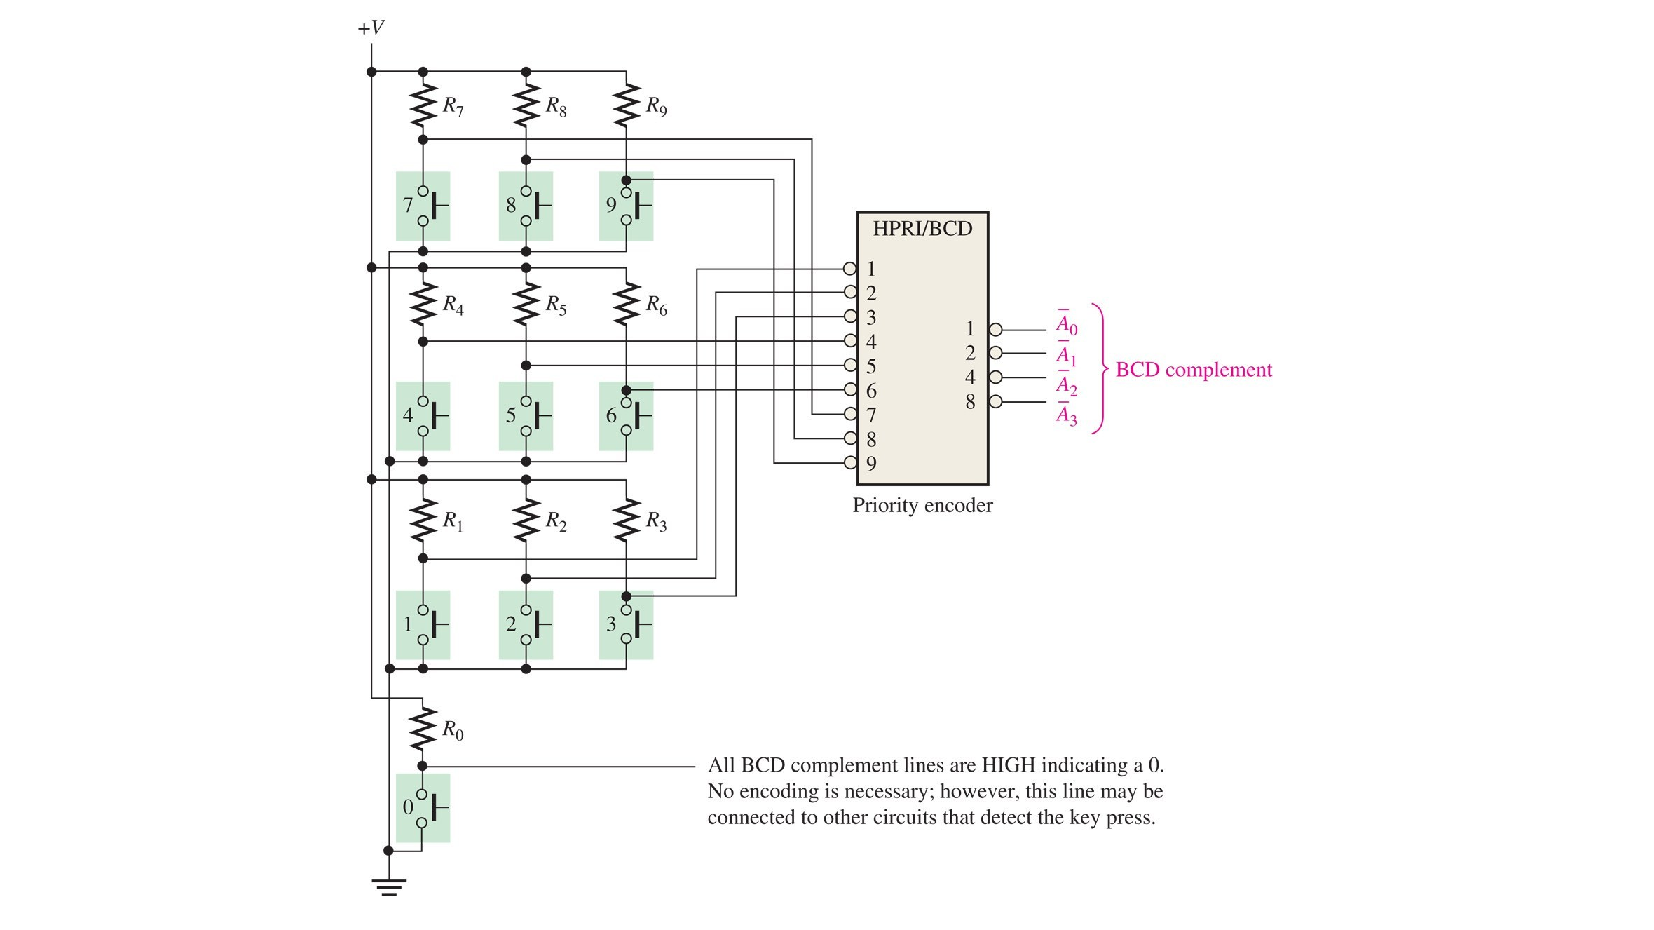
\includegraphics[width=0.75\textwidth,trim=3cm 0cm 3cm 0cm,clip=true]{figures/encoder2.pdf}
\caption{\label{fig:house} Resistors in parallel arranged in a keypad system.}
\end{figure}
\end{frame}

\section{PhET Activity: Series and Parallel Resistors}

\begin{frame}{PhET Activity: DC Circuits and Ohm's Law}
\footnotesize
\textbf{How do we deal with complex circuits?}
\begin{enumerate}
\item Create a circuit that involves four identical resistors \textit{in series}.
\item Use an ammeter to show that the current is the same in all resistors.
\item Calculate the \textit{effective total resistance} by plotting an $i-V$ curve of the system.  Measure $i$ and $V$ by changing the voltage and using the voltmeter and ammeter.  Does the slope of the $i-V$ curve match your expectation?
\item Create a circuit that involves four identical resistors \textit{in parallel}.
\item Use the voltmeter to show that the change in voltage is the same across all resistors.
\item Calculate the \textit{effective total resistance} by plotting an $i-V$ curve of the system.  Measure $i$ and $V$ by changing the voltage and using the voltmeter and ammeter.   Does the slope of the $i-V$ curve match your expectation?
\end{enumerate}
\end{frame}

\section{Electromotive Force (EMF) and Terminal Voltage}

\begin{frame}{Electromotive Force (EMF) and Terminal Voltage}
\small
\textbf{\alert{The electromotive force (EMF)}} of a battery is the potential difference that induces current through the circuit.  It is \textit{almost} the same as the battery voltage.
\begin{figure}
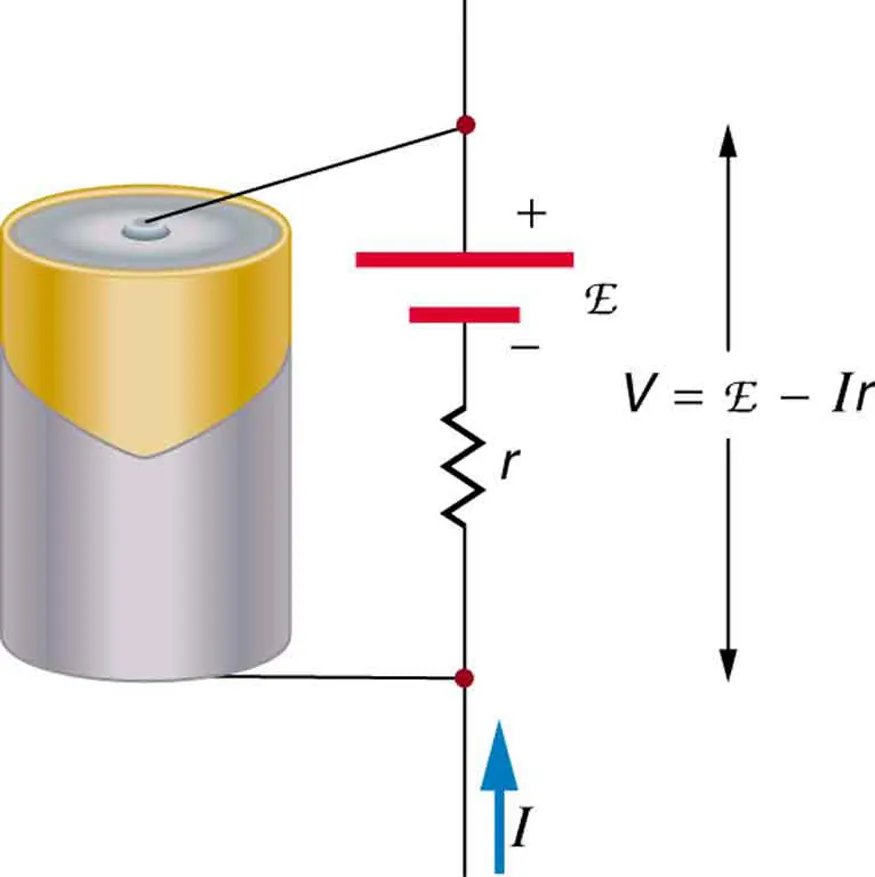
\includegraphics[width=0.45\textwidth]{figures/internal_r.png}
\caption{\label{fig:internal_r} \textit{Internal resistance} is one internal property of a battery.}
\end{figure}
\end{frame}

\begin{frame}{Electromotive Force (EMF) and Terminal Voltage}
\small
\textbf{\alert{The electromotive force (EMF)}} of a battery is the potential difference that induces current through the circuit.
\begin{figure}
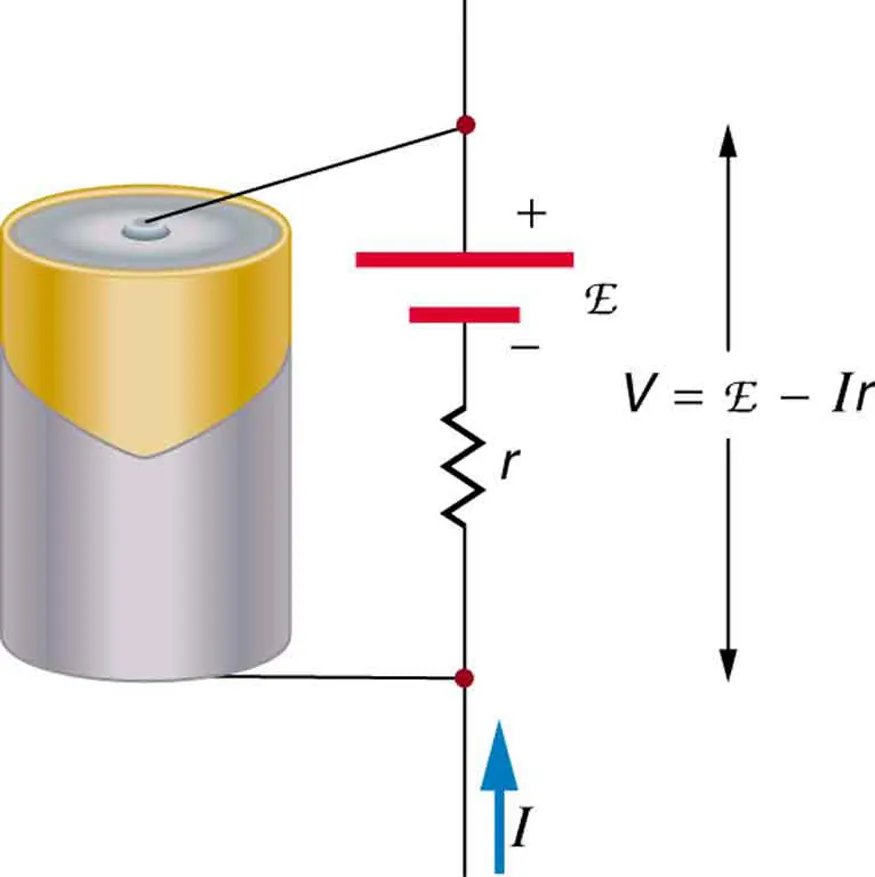
\includegraphics[width=0.25\textwidth]{figures/internal_r.png} \hspace{0.25cm}
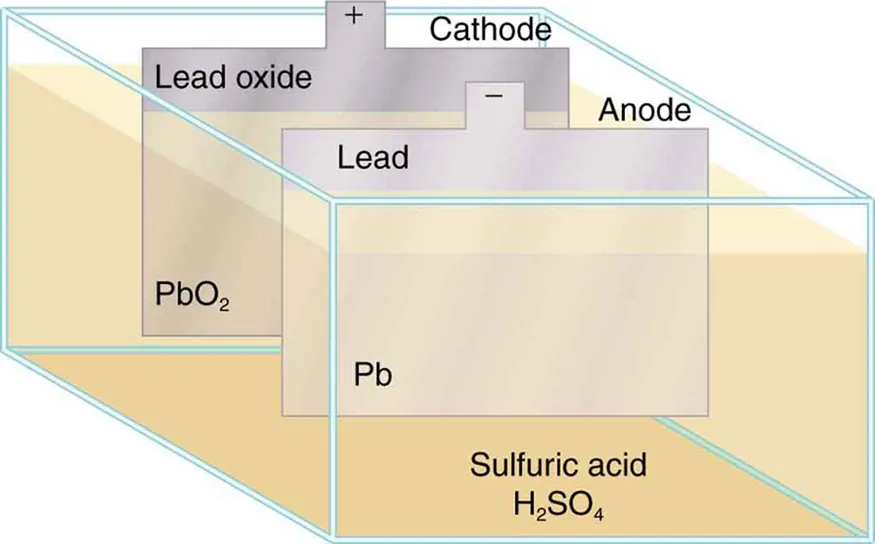
\includegraphics[width=0.33\textwidth]{figures/internal_batt_1.png}
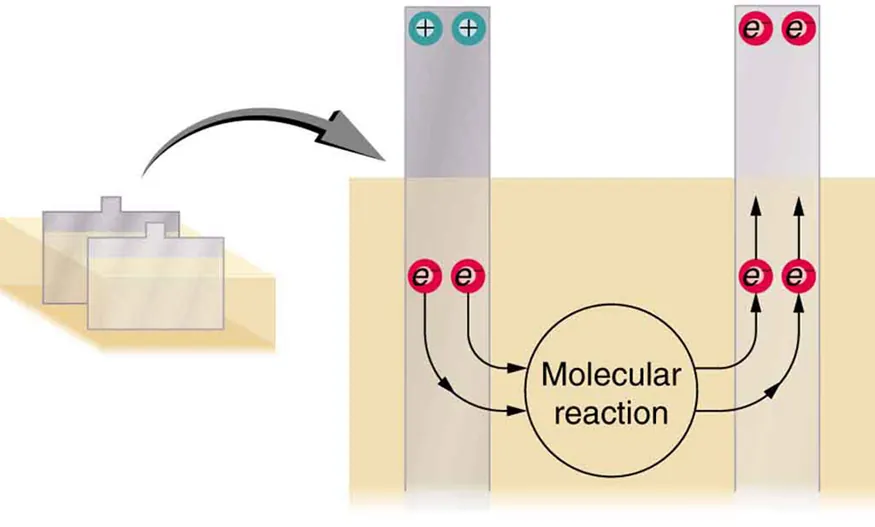
\includegraphics[width=0.33\textwidth]{figures/internal_batt_2.png}
\caption{\label{fig:internal_r2} \textit{Internal resistance} arises from battery chemistry, designed to pull electrons from the cathode to the anode before terminal connection.}
\end{figure}
\begin{equation}
V_{\rm out} = \mathcal{E} - I r
\end{equation}
\end{frame}

\begin{frame}{Electromotive Force (EMF) and Terminal Voltage}
\small
\textbf{\alert{The electromotive force (EMF)}} of a battery is the potential difference that induces current through the circuit.
\begin{figure}
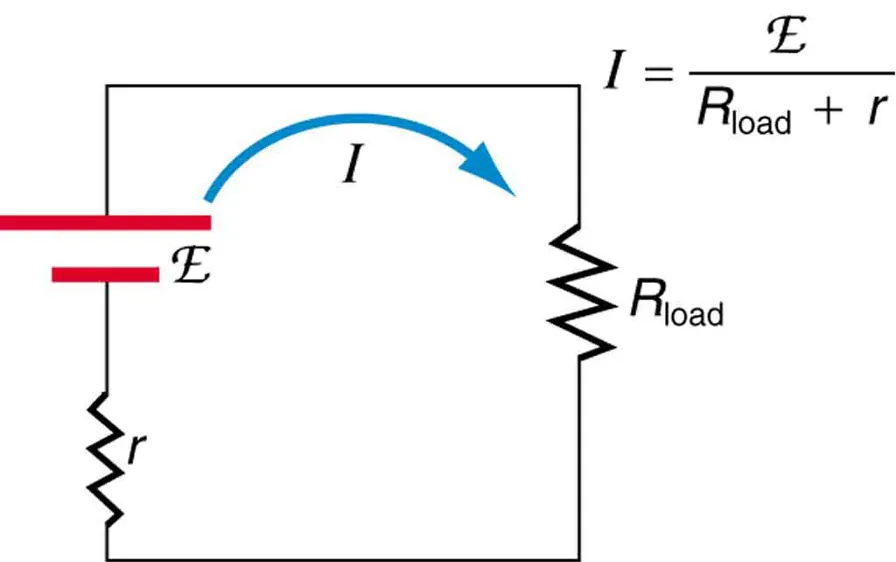
\includegraphics[width=0.45\textwidth]{figures/internal_batt_3.png}
\caption{\label{fig:internal_r3} \textit{Internal resistance} is one internal property of a battery.}
\end{figure}
\begin{equation}
I = \frac{\mathcal{E}}{R_{\rm load} + r}
\end{equation} \\ \vspace{0.5cm}
Reduces to Ohm's law if $r$ is insignificant.
\end{frame}

\begin{frame}{Electromotive Force (EMF) and Terminal Voltage}
If we treat the internal resistance of a 3.3 V battery as 0 $\Omega$, and we connect $R_{\rm load} = 100 \Omega$ in a simple circuit, what will be the current?
\begin{itemize}
\item A: 3.3 A
\item B: 3.3 mA
\item C: 33 mA
\item D: 33 A
\end{itemize}
\footnotesize{Hint: draw the circuit if you are not sure.}
\end{frame}

\begin{frame}{Electromotive Force (EMF) and Terminal Voltage}
Internal resistance tends to rise if the battery is depleted of chemical energy.  If we treat the internal resistance of a 3.3 V battery as 10 $\Omega$, and we connect $R_{\rm load} = 100 \Omega$ in a simple circuit, what will be the current?
\begin{itemize}
\item A: 3.3 A
\item B: 3.3 mA
\item C: 30 mA
\item D: 30 A
\end{itemize}
\footnotesize{Hint: draw the circuit if you are not sure.}
\end{frame}

\begin{frame}{Electromotive Force (EMF) and Terminal Voltage}
Suppose we have a device that operates at 9V, and we have a 9V battery with $r = 1 \Omega$.  If we connect a $9 \Omega$ load resistance, what will be the terminal voltage?  Will the device operate normally?
\begin{itemize}
\item A: 8.1V
\item B: 8V
\item C: 9.1V
\item D: 9V
\end{itemize}
\footnotesize{Will the device operate normally?}
\end{frame}

\begin{frame}{Electromotive Force (EMF) and Terminal Voltage}
In the previous problem, what fraction of the power is disspated in the internal resistor?  \\ \vspace{0.5cm}
\footnotesize
 \textit{Hint: think of dissipated power as $P = I^2 R$ and $P = I^2 r$ for the load and internal resistance, respectively.}
 \normalsize
\begin{itemize}
\item A: 5\%
\item B: 10\%
\item C: 1\%
\item D: 11\%
\end{itemize}
\end{frame}

\begin{frame}{Electromotive Force (EMF) and Terminal Voltage}
\small
\textbf{\alert{Connecting real batteries in series}} raises the effective terminal voltage, but there are now two internal resistances.
\begin{figure}
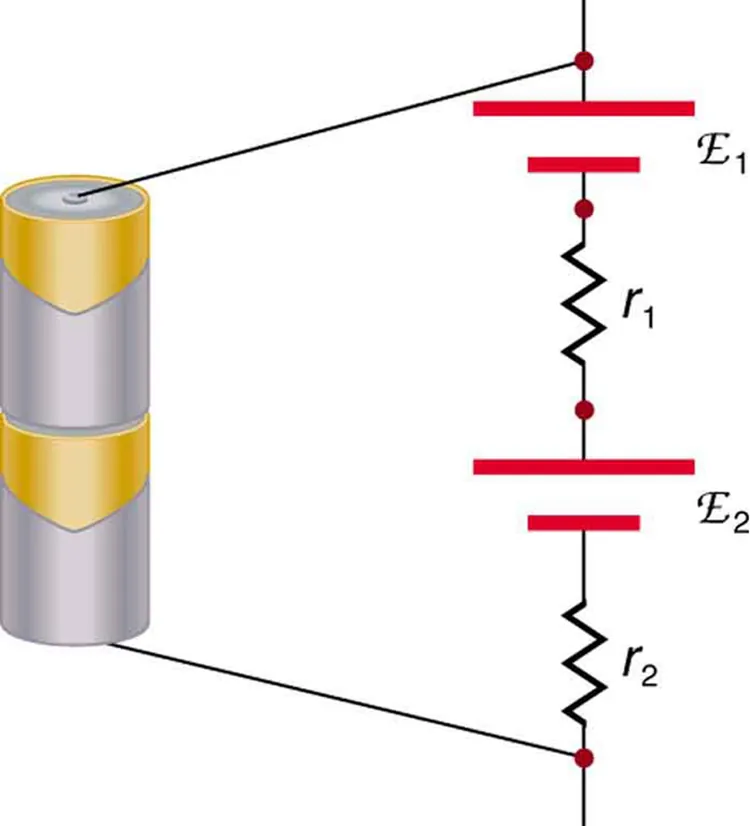
\includegraphics[width=0.25\textwidth]{figures/internal_batt_4.png} \hspace{1cm}
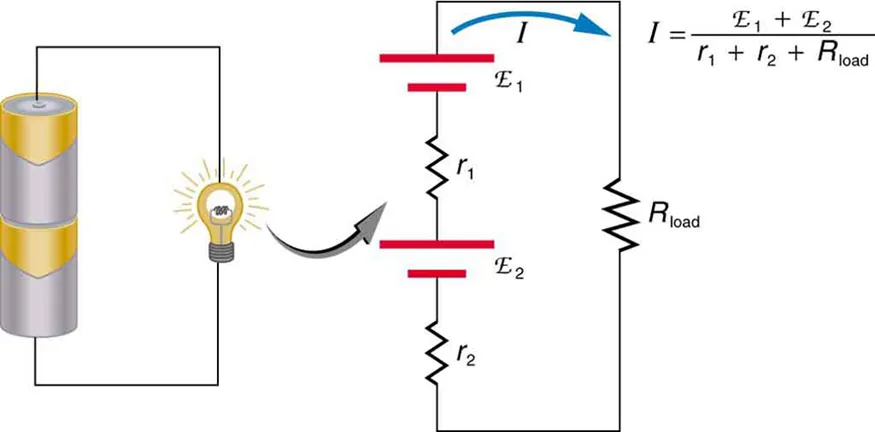
\includegraphics[width=0.55\textwidth]{figures/internal_batt_5.png}
\caption{\label{fig:internal_r4} (Left) Two batteries in series. (Right) Two batteries in series connected to a load resistance.}
\end{figure}
\begin{equation}
I = \frac{\mathcal{E}_1 + \mathcal{E}_2}{R_{\rm load} + r_1 + r_2}
\end{equation}
\end{frame}

\begin{frame}{Electromotive Force (EMF) and Terminal Voltage}
Suppose we have a flashlight powered by four AA batteries \textit{in series.}  The EMF of each AA battery is 1.5V.  The internal resistance is $r = 0.5\Omega$ for each battery.  The load resistance of the flashlight bulb is $30 \Omega$.  What is the current flow?
\begin{itemize}
\item A: $1.67$ A
\item B: $0.167$ A
\item C: $0.2$ A
\item D: $2.0$ A
\end{itemize}
\footnotesize{Remember to draw a picture of the whole circuit if you are stuck.}
\end{frame}

\begin{frame}{Electromotive Force (EMF) and Terminal Voltage}
Suppose we have a flashlight powered by four AA batteries \textit{in series.}  The EMF of each AA battery is 1.5V.  The internal resistance is $r = 0.5\Omega$ for each battery.  The load resistance of the flashlight bulb is $30 \Omega$.  What is the terminal voltage?
\begin{itemize}
\item A: $6.0$ V
\item B: $1.5$ V
\item C: $3.33$ V
\item D: $5.67$ V
\end{itemize}
\footnotesize{Remember to draw a picture of the whole circuit if you are stuck.}
\end{frame}

\section{Kirchhoff's Rules}

\begin{frame}{Kirchhoff's Rules}
\small
\begin{tcolorbox}[colback=white,colframe=gray,title=Kirchhoff's Rules]
\alert{The following two rules govern complex circuits:
\begin{itemize}
\item The sum of all currents entering a junction must equal the sum of all currents leaving the junction: $\sum_n I_{\rm n,in} = \sum_n I_{\rm n,out}$.
\item The algebraic sum of changes in potential around any closed loop must be zero: $\sum_{n,loop} V_n = 0$.
\end{itemize}}
\end{tcolorbox}
\begin{itemize}
\item The first rule follows from charge conservation, and is called the \textit{junction rule}.
\item The second rule follows from energy conservation, and is called the \textit{loop rule.}
\end{itemize}
\end{frame}

\begin{frame}{Kirchhoff's Rules}
\small
\textbf{\alert{Kirchhoff's rules help organize calculations}} for complex circuits.
\begin{figure}
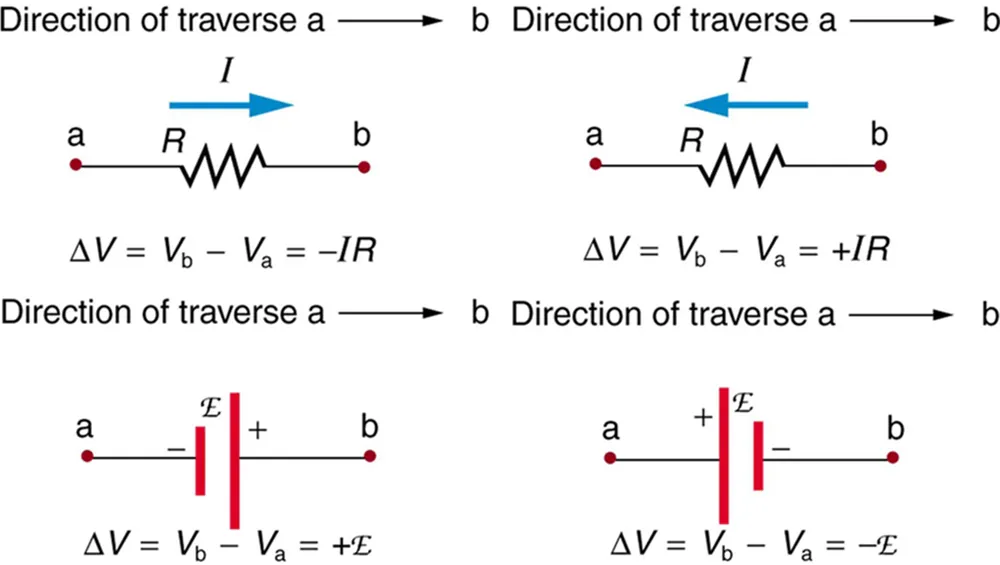
\includegraphics[width=0.5\textwidth]{figures/complex_2.png} \hspace{1cm}
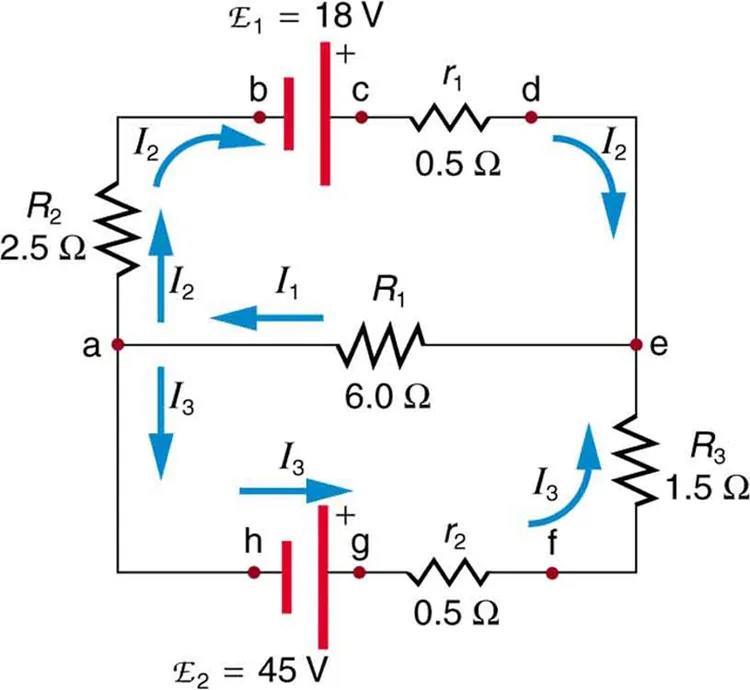
\includegraphics[width=0.35\textwidth]{figures/complex_1.png}
\caption{\label{fig:kirch1} (Left) A change in voltage across a resistor is negative in the direction of current flow.  The change is positive if aligned with the polarity of the battery. (Right) The complex circuit has two loops, three load resistors, two batteries, and two internal resistances.}
\end{figure}
\end{frame}

\begin{frame}{Kirchhoff's Rules}
\small
\textbf{\alert{Kirchhoff's rules help organize calculations}} for complex circuits.
\begin{figure}
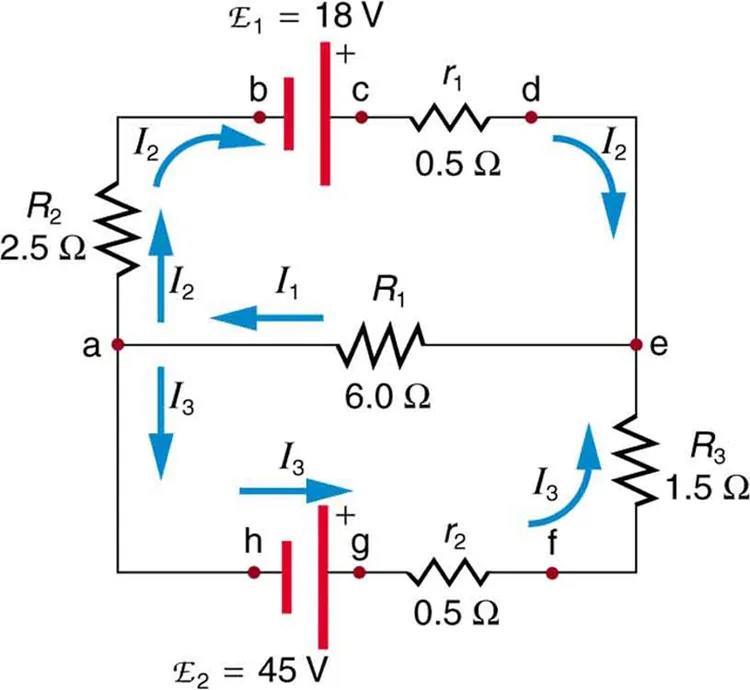
\includegraphics[width=0.5\textwidth]{figures/complex_1.png}
\caption{\label{fig:kirch2} (a) Solve this one in small groups. (b) Model this in DC Circuit Constructor PhET.}
\end{figure}
\end{frame}

\section{Voltmeters and Ammeters}

\begin{frame}{Voltmeters and Ammeters}
\textbf{\alert{A galvanometer}} is a device that deflects a needle based on the strength of a current.  Galvanometers can be used to create \textit{voltmeters} and \textit{ammeters}.
\footnotesize
\begin{figure}
\centering
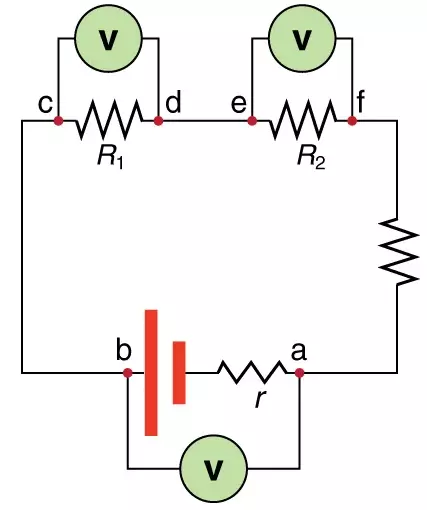
\includegraphics[width=0.3\textwidth]{figures/voltmeter.png} \hspace{0.5cm}
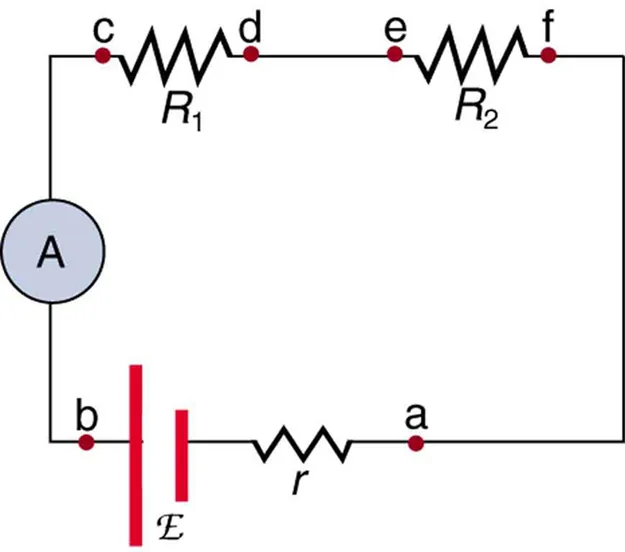
\includegraphics[width=0.3\textwidth]{figures/ammeter.png}
\caption{\label{fig:meas} (Left) A voltmeter is connected in parallel. (Right) An ammeter is connected in series.  These connections are necessary to make the measurements.}
\end{figure}
\end{frame}

\begin{frame}{Voltmeters and Ammeters}
\textbf{\alert{A galvanometer}} is a device that deflects a needle based on the strength of a current.  This effect is caused by the force of a magnetic field on a current-carrying wire.
\footnotesize
\begin{figure}
\centering
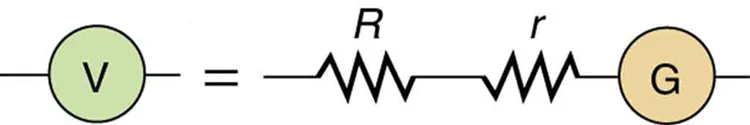
\includegraphics[width=0.45\textwidth]{figures/galvo_1.png} \hspace{0.5cm}
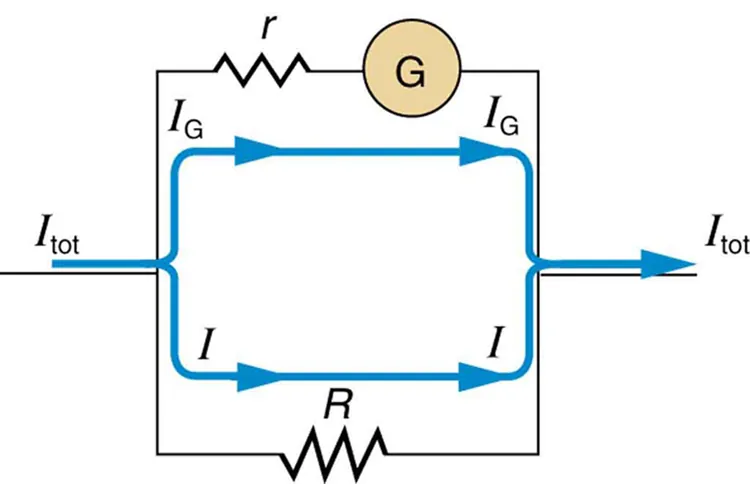
\includegraphics[width=0.45\textwidth]{figures/galvo_2.png}
\caption{\label{fig:galvo} (Left) A galvonometer (G) within a voltmeter is protected by a large resistor, $R$.  (Right) A galvonometer (G) within an ammeter is protected by a large resistor, $R$.  Each G has an internal resistance, $r$.  The value of $R$ also calibrates the measurement in both situations.}
\end{figure}
\end{frame}

\begin{frame}{Voltmeters and Ammeters}
\small
\textbf{\alert{Suppose}} the ammeter below has an internal resistance $r = 10\Omega$, and a ``shunt'' resistance of $R = 0.1\Omega$, $R_1 = 1$ k$\Omega$, $R_2 = 1$ k$\Omega$, and the battery has $\mathcal{E} = 12$V and an internal resistance of $r_b = 1 \Omega$.
\footnotesize
\begin{figure}
\centering
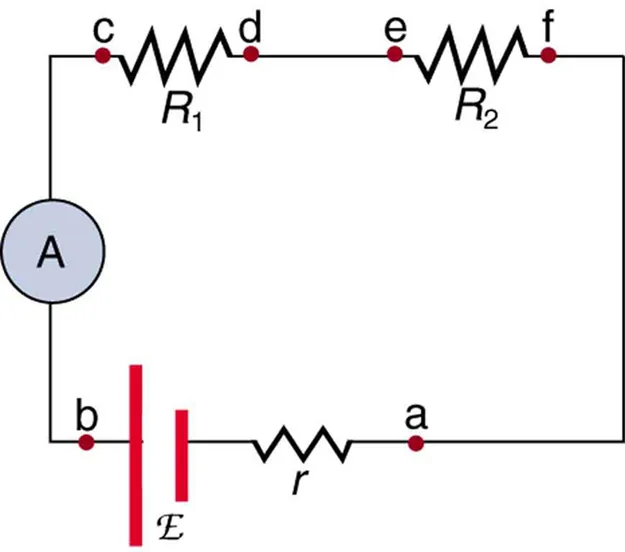
\includegraphics[width=0.35\textwidth]{figures/ammeter.png} \hspace{0.5cm}
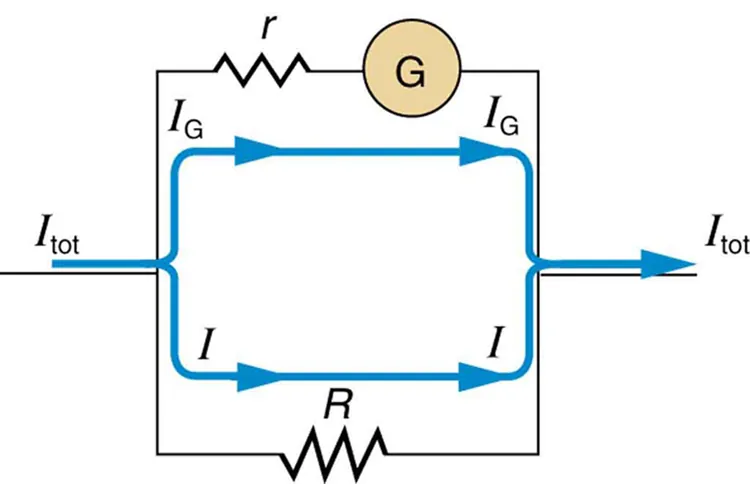
\includegraphics[width=0.45\textwidth]{figures/galvo_2.png}
\caption{\label{fig:galvo2} (Left) An ammeter connceted in series with loads represented by $R_1$ and $R_2$, and a battery with emf $\mathcal{E}$ and internal resistance $r_b$. (Right) The internal structure of the ammeter, with galvanometer G, internal resistance $r$ and shunt resistance $R$.}
\end{figure}
\end{frame}

\begin{frame}{Voltmeters and Ammeters}
\small
\textbf{\alert{Suppose}} the ammeter below has an internal resistance $r = 10\Omega$, and a ``shunt'' resistance of $R = 0.1\Omega$, $R_1 = 0.5$ k$\Omega$, $R_2 = 0.5$ k$\Omega$, and the battery has $\mathcal{E} = 12$V and an internal resitance of $r_b = 1 \Omega$.
\begin{enumerate}
\item Calculate the total resistance of the ammeter, $R_{\rm A}$.
\item Calculate the total current flow from the battery, $I_{\rm total}$.
\item What is the decrease in voltage across the ammeter?
\item What is the current flow to G, the galvanometer, $I_{\rm G}$?
\end{enumerate}
\textbf{Solve each of these exercises in small groups.}  \textit{Does the shunt resistor draw more current than G?}  After we have solutions, we can model the current flow in the DC Circuits PhET.
\end{frame}

\begin{frame}{Voltmeters and Ammeters}
\small
\textbf{\alert{Suppose}} the voltmeter below has an internal resistance $r = 10\Omega$, and a ``blocking'' resistance of $R = 100$ k$\Omega$, $R_1 = 0.5$ k$\Omega$, $R_2 = 0.5$ k$\Omega$, and the battery has $\mathcal{E} = 12$V and an internal resitance of $r_b = 1 \Omega$.
\footnotesize
\begin{figure}
\centering
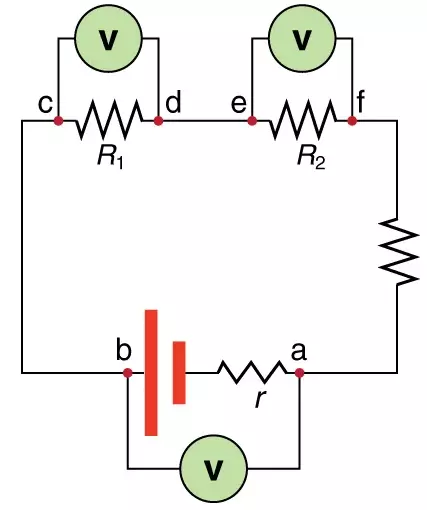
\includegraphics[width=0.3\textwidth]{figures/voltmeter.png} \hspace{0.5cm}
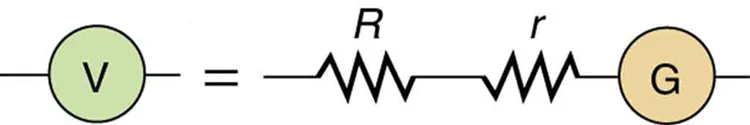
\includegraphics[width=0.45\textwidth]{figures/galvo_1.png}
\caption{\label{fig:galvo3} (Left) The voltmeter probes spots in the DC circuit.  Assume there is no third resistor after $R_2$.  (Right) The voltmeter has a galvanometer, G, a blocking resistor $R$, and internal resistance $r$.}
\end{figure}
\end{frame}

\begin{frame}{Voltmeters and Ammeters}
\small
\textbf{\alert{Suppose}} the voltmeter below has an internal resistance $r = 10\Omega$, and a ``blocking'' resistance of $R = 100$ k$\Omega$, $R_1 = 0.5$ k$\Omega$, $R_2 = 0.5$ k$\Omega$, and the battery has $\mathcal{E} = 12$V and an internal resitance of $r_b = 1 \Omega$.
\begin{enumerate}
\item What is the effective resistance of the voltmeter?
\item What is the resistance of the voltmeter combined in parallel with $R_{1}$?
\item What is the current flow, $I$, from the battery?
\item What is the voltage decrease across the $R_1$ plus voltmeter complex?
\item What is the current flow to G, the galvanometer, $I_{\rm G}$?
\end{enumerate}
\textbf{Solve each of these exercises in small groups.}  \textit{Does the shunt resistor draw more current than G?}  After we have solutions, we can model the current flow in the DC Circuits PhET.
\end{frame}

\section{RC Circuits}

\begin{frame}{RC Circuits}
\textbf{\alert{An RC circuit}} is a simply connected circuit that has resistance and capacitance.
\begin{figure}
\centering
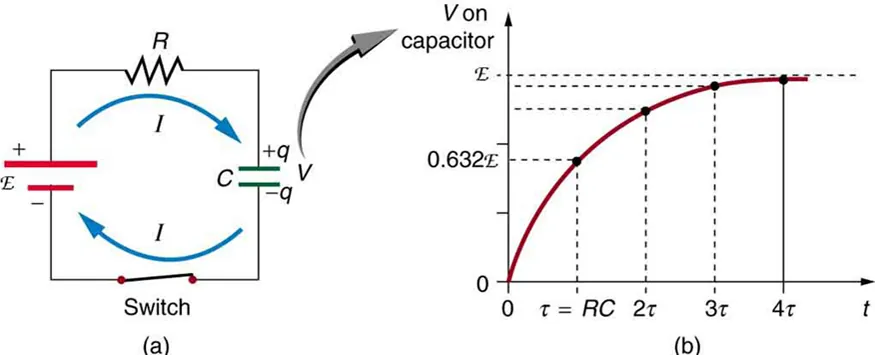
\includegraphics[width=0.8\textwidth]{figures/RC_1.png}
\caption{\label{fig:RC1} (Left) A battery with emf $\mathcal{E}$ induces current through $R$ and charges $C$.  (Right) The voltage on the capacitor versus time.  Note that $RC$ has units of time.}
\end{figure}
\end{frame}

\begin{frame}{RC Circuits}
\textbf{\alert{An RC circuit}} is a simply connected circuit that has resistance and capacitance.
\begin{figure}
\centering
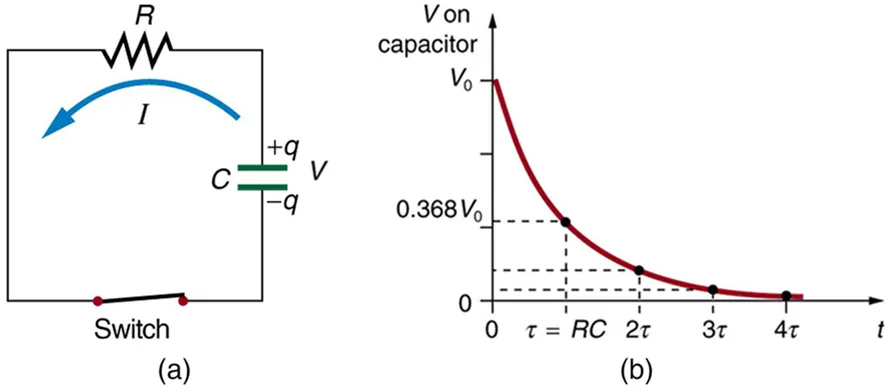
\includegraphics[width=0.8\textwidth]{figures/RC_2.png}
\caption{\label{fig:RC2} (Left) A charged capacitor induces current through $R$.  (Right) The voltage on the capacitor versus time.  Note that $RC$ has units of time.}
\end{figure}
\end{frame}

\begin{frame}{RC Circuits}
\begin{tcolorbox}[colback=white,colframe=gray,title=RC Circuit Equations]
\alert{Let $R$ and $C$ be the resitance and capacitance in an RC circuit, let $\tau = RC$ be the time constant, and let $\mathcal{E}$ be the emf when charging.  The following two equations may be proven for RC cicuits:
\begin{align}
V_{\rm C} =& \mathcal{E}\left(1 - e^{-t/\tau}\right) \\
V_{\rm C} =& \mathcal{E}e^{-t/\tau}
\end{align}}
\end{tcolorbox}
\end{frame}

\begin{frame}{RC Circuits}
Suppose an RC circuit is built from a 1 k$\Omega$ resistor, a 1 $\mu$F capacitor, and a 5 V battery.  What is the time constant?
\begin{itemize}
\item A: 1 second
\item B: 0.1 seconds
\item C: 0.01 seconds
\item D: 1 ms
\end{itemize}
\end{frame}

\begin{frame}{RC Circuits}
Suppose the same RC circuit is connected and charges.  What is the voltage on the capacitor after $t = 10\tau$?
\begin{itemize}
\item A: 5V
\item B: 4.9V
\item C: 2.5V
\item D: 0V
\end{itemize}
\end{frame}

\begin{frame}{RC Circuits}
Suppose the same charged RC circuit is disconnected from the battery and connected to a load.  What is the voltage on the capacitor after $t = 10\tau$?
\begin{itemize}
\item A: 5V
\item B: 4.9V
\item C: 2.5V
\item D: 0V
\end{itemize}
\end{frame}

\begin{frame}{RC Circuits}
After two time constants, what percentage of the final voltage, emf, is on an initially uncharged capacitor C, charged through a resistance R?
\begin{itemize}
\item A: 13.2 percent
\item B: 26.7 percent
\item C: 86.5 percent
\item D: 99.5 percent
\end{itemize}
\end{frame}

\begin{frame}{RC Circuits}
\small
\textbf{\alert{Think back}} to the prior unit, when we explored capacitance.  Which of the circuits in Fig. \ref{fig:three_cap} takes longer to charge and discharge?  Explain why this is true in terms of $\tau = RC$. (Group discussion).  \textbf{We will now construct and test an RC circuit.}
\begin{figure}
\centering
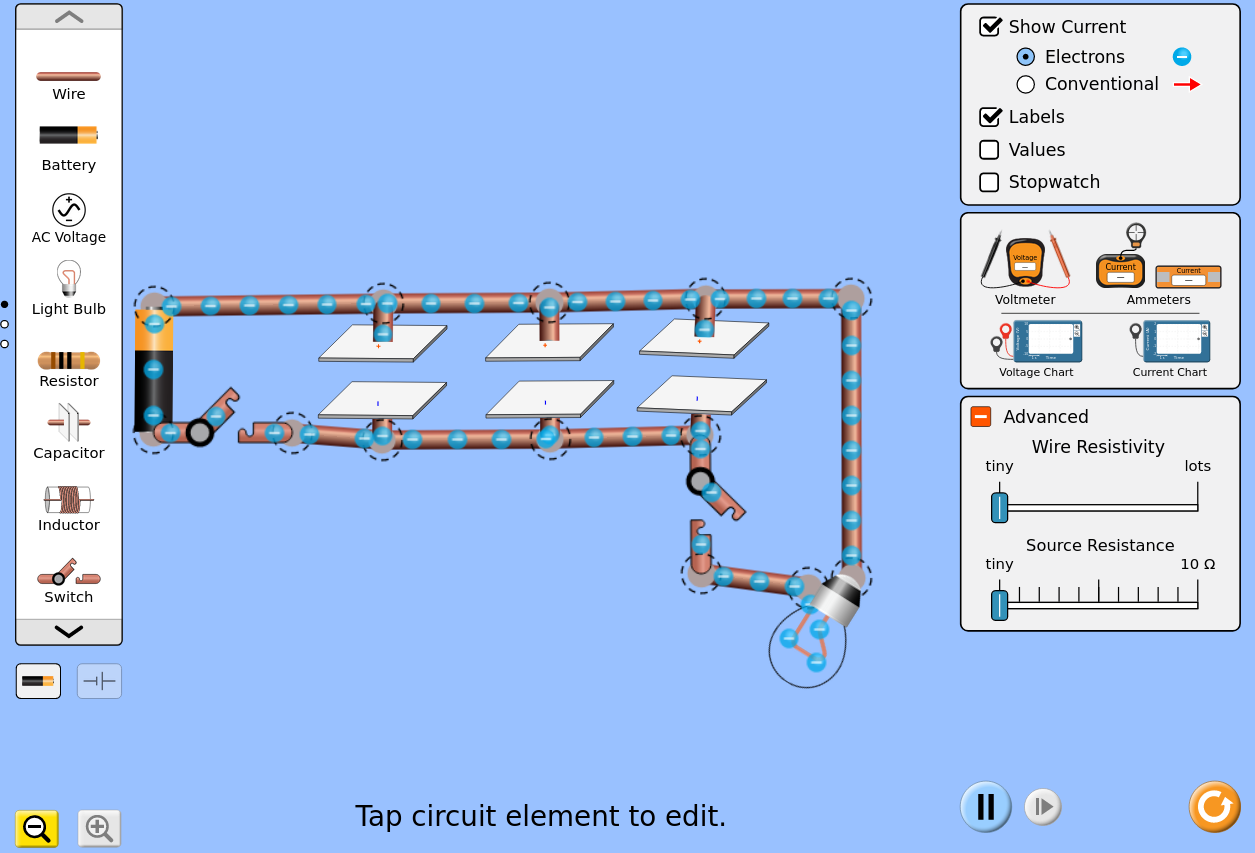
\includegraphics[width=0.45\textwidth]{figures/three_cap_2.png}
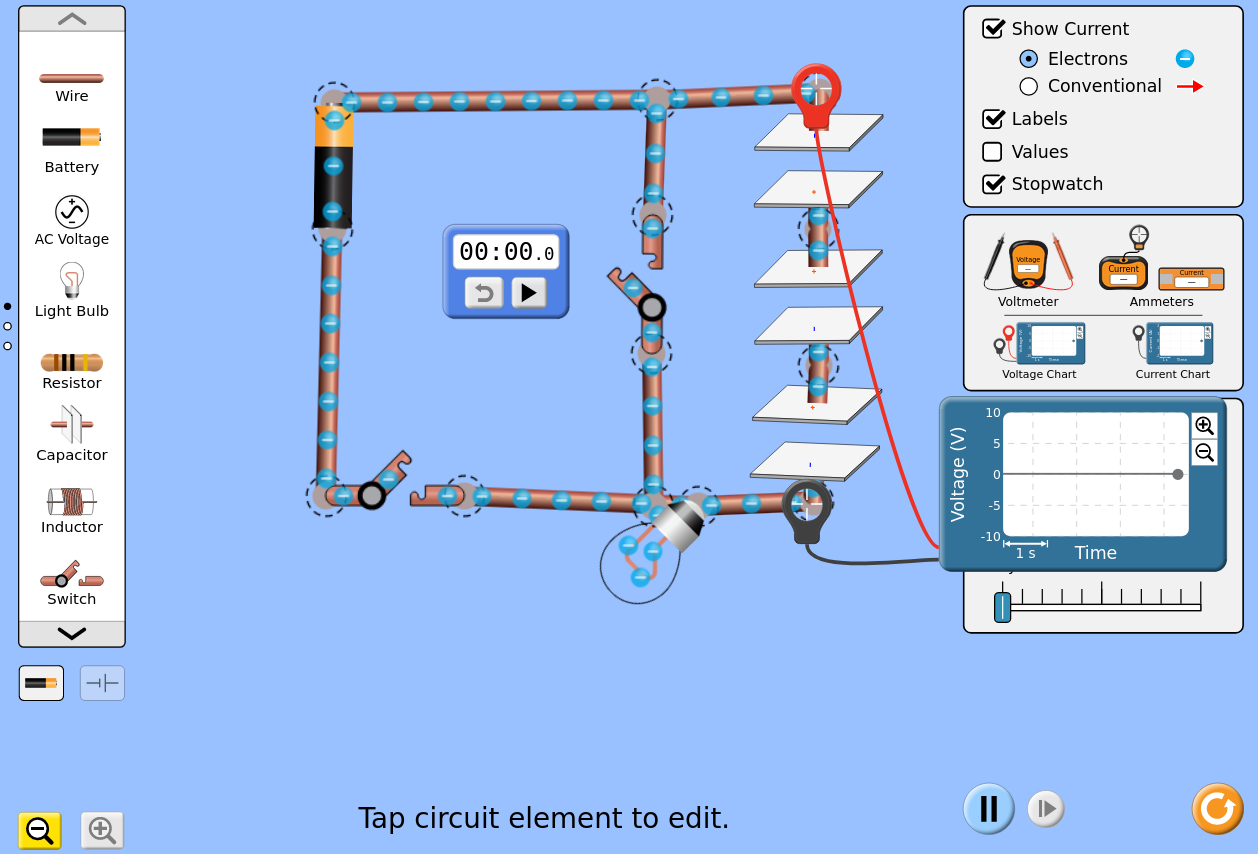
\includegraphics[width=0.45\textwidth]{figures/three_cap_3.png}
\caption{\label{fig:three_cap} (Left) Three identical capacitors are charged in parallel. (Right) Three identical capacitors are charged in series.}
\end{figure}
\end{frame}

\section{Conclusion}

\begin{frame}{Unit 2 Summary}
\textbf{Reading: Chapters 21.1 - 21.4, 21.6}
\begin{enumerate}
\item Resistors in series and parallel
\item Electromotive force (EMF) and terminal voltage
\item Kirchhoff's rules
\item Voltmeters and ammeters
\item RC circuits
\end{enumerate}
\end{frame}

\end{document}
